\documentclass[10pt]{article}
\usepackage[top=3cm, bottom=4cm, left=3.5cm, right=3.5cm]{geometry}
\usepackage{amsmath,amsthm,amsfonts,amssymb,amscd, fancyhdr, color, comment, graphicx, environ}
\usepackage{float}
\usepackage{mathrsfs}
\usepackage[math-style=ISO]{unicode-math}
\setmathfont{TeX Gyre Termes Math}
\usepackage{lastpage}
\usepackage[dvipsnames]{xcolor}
\usepackage[framemethod=TikZ]{mdframed}
\usepackage{enumerate}
\usepackage[shortlabels]{enumitem}
\usepackage{fancyhdr}
\usepackage{indentfirst}
\usepackage{listings}
\usepackage{sectsty}
\usepackage{thmtools}
\usepackage{shadethm}
\usepackage{hyperref}
\usepackage{setspace}
\hypersetup{
    colorlinks=true,
    linkcolor=blue,
    filecolor=magenta,      
    urlcolor=blue,
}
\usepackage[makeroom]{cancel}
\usepackage[utf8]{inputenc}
\usepackage[T1]{fontenc}
\usepackage{hyperref}
\hypersetup{colorlinks=true, linkcolor=blue, filecolor=magenta, urlcolor=cyan,}
\urlstyle{same}
\usepackage{amsmath}
\usepackage{amsfonts}
\usepackage{amssymb}
\usepackage[version=4]{mhchem}
\usepackage{stmaryrd}
\usepackage{graphicx}
\usepackage{subcaption}
\usepackage[export]{adjustbox}
\graphicspath{ {./images/} }
\usepackage{listings}
\hypersetup{colorlinks=true, linkcolor=blue, filecolor=magenta, urlcolor=cyan,}
\urlstyle{same}

\title{CS5785 Homework 4 }

\author{}
\date{}


\begin{document}
\maketitle
The homework has two parts: programming exercises and written exercises.

This homework is due on Nov 21, 2023 at 11:59 PM ET. Upload your homework to Gradescope (Canvas->Gradescope). There are two assignments for this homework in Gradescope. Please note a complete submission should include:

\begin{enumerate}
  \item A write-up as a single .pdf file, which should be submitted to "Homework 4 (write-up)" This file should contain your answers to the written questions and exported pdf file / structured write-up of your answers to the coding questions (which should include core codes, plots, outputs, and any comments / explanations). We will deduct points if you do not do this.

  \item Source code for all of your experiments (AND figures) zipped into a single .zip file, in . py files if you use Python or .ipynb files if you use the IPython Notebook. If you use some other language, include all build scripts necessary to build and run your project along with instructions on how to compile and run your code. If you use the IPython Notebook to create any graphs, please make sure you also include them in your write-up. This should be submitted to "Homework 4 (code)".

  \item You need to mark the pages of your submission to each question on Gradescope after submission, Gradescope should ask you to do that after you upload your write-up by default. We might deduct points if you do not do this.

\end{enumerate}

The write-up should contain a general summary of what you did, how well your solution works, any insights you found, etc. On the cover page, include the class name, homework number, and team member names. You are responsible for submitting clear, organized answers to the questions. You could use online $\mathrm{AT}_{\mathrm{EX}} \mathrm{X}$ templates from Overleaf, under "Homework Assignment" and and "Project / Lab Report". You could also use a $\mathrm{AT}_{\mathrm{EX}} \mathrm{X}$ template we made, which contains useful packages for writing math equations and code snippet.

Please include all relevant information for a question, including text response, equations, figures, graphs, output, etc. If you include graphs, be sure to include the source code that generated them. Please pay attention to Canvas for relevant information regarding updates, tips, and policy changes. You are encouraged (but not required) to work in groups of 2.

\section*{IF YOU NEED HELP}
There are several strategies available to you.

\begin{itemize}
  \item If you get stuck, we encourage you to post a question on the Discussions section of Canvas. That way, your solutions will be available to other students in the class.

  \item The professor and TAs offer office hours, which are a great way to get some one-on-one help.

  \item You are allowed to use well known libraries such as scikit-learn, scikit-image, numpy, scipy,
etc. for this assignment (including implementations of machine learning algorithms), unless we explicitly say that you cannot in a particular question. Any reference or copy of public code repositories should be properly cited in your submission (examples include Github, Wikipedia, Blogs).

\end{itemize}

\section*{PROGRAMMING EXERCISES}
\section*{1. Convolutional Neural Networks}
We will work with the MNIST dataset for this question. This dataset contains 60,000 training images of handwritten numbers from 0 to 9 , and you need to recognize the handwritten numbers by building a CNN.

You will use the Keras library for this. You might have to install the library if it hasn't been installed already. Please check the installation by printing out the version of Keras inside the python shell as follows.

import keras

keras.\_\textit{version}-

The above lines will give you the current version of Keras you are using. Once this works, you can proceed with the assignment.

(a) Loading Dataset For using this dataset, you will need to import mnist and use it as follows.

from keras.datasets import mnist

(train\_X, train\_Y), (test\_X, test\_Y) = mnist.load\_data $($ )

To verify that you have loaded the dataset correctly, try printing out the shape of your train and test dataset matrices. Also, try to visualize individual images in this dataset by using imshow() function in pyplot. Below are some example images from the Tensorflow datasets catalog.

\begin{center}
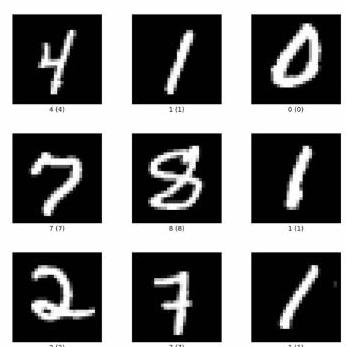
\includegraphics[max width=\textwidth]{2023_11_03_3a37fc63330e1b210712g-2}
\end{center}

(b) Preprocessing The data has images with $28 \times 28$ pixel values. Since we use just one grayscale color channel, you need to reshape the matrix such that we have a $28 \times 28 \times 1$ sized matrix holding each input data-point in the training and testing dataset. The output variable can be converted into a one-hot vector by using the function to\_categorical (make sure you import to\_categorical from keras.utils). For example, if the output label for a given image is the digit 2 , then the one-hot representation for this consists of a 10 -element vector, where the element at index 2 is set to 1 and all the other elements are zero.

For preprocessing, scale the pixel values such that they lie between 0.0 and 1.0. Make sure that you use the appropriate conversion to float wherever required while scaling.

You can include all these steps into a single python function that loads your dataset appropriately. Once you finish this, visualize some images using imshow() function.

(c) Implementation

Now, to define a CNN model, we will use the Sequential module in Keras. We are providing you with the code for creating a simple CNN here. We use Conv2D (for declaring 2D convolutional networks), MaxPooling2D (for maxpooling layer), Dense (for densely connected neural network layers) and Flatten (for flattening the input for next layer).

\begin{lstlisting}[language=Python]
from keras.models import Sequential
from keras.layers import Conv2D
from keras.layers import MaxPooling2D
from keras.layers import Dense
from keras.layers import Flatten
from keras.optimizers import SGD

def create\_cnn():

\# define using Sequential

model $=$ Sequential $($ )

\# Convolution layer

model.add (

Conv2D $(32,(3,3)$,

activation $=$ 'relu ',

kernel\_initializer='he\_uniform ' , input\_shape $=(28,28,1))$

)

\# Maxpooling layer

model .add (MaxPooling2D ((2, 2) ) )

\# Flatten output

model.add (Flatten ())

\# Dense layer of 100 neurons

model.add (

Dense $(100$,

activation $=$ ' relu ',

kernel\_initializer='he\_uniform ' )

)

model. $\operatorname{add}($ Dense $(10$, activation $=$ 'softmax ' $))$

\# initialize optimizer

opt $=\operatorname{SGD}(1 \mathrm{r}=0.01$, momentum $=0.9)$

\# compile model

model.compile (

optimizer=opt ,

loss='categorical\_crossentropy',

metrics $=[$ 'accuracy' $]$

)

return model
\end{lstlisting}

Specifically, we have added the following things in this code.
i. A single convolutional layer with $3 \times 3$ sized window for computing the convolution, with 32 filters

ii. Maxpooling layer with $2 \times 2$ window size.

iii. Flatten resulting features to reshape your output appropriately.

iv. Dense layer on top of this (100 neurons) with ReLU activation

v. Dense layer with 10 neurons for calculating softmax output (Our classification result will output one of the ten possible classes, corresponding to our digits)

After defining this model, we use Stochastic Gradient Descent (SGD) optimizer and crossentropy loss to compile the model. We are using a learning rate of 0.01 and a momentum of 0.9 here. We have added this to the given code stub already. Please see that this code stub works for you. Try to print model.layers in your interactive shell to see that the model is generated as we defined.

\section*{(d) Training and Evaluating CNN}
Now we will train the network. You can see some examples here. Look at the fit() and evaluate() methods.

You will call the fit method with a validation split of 0.1 (i.e. $10 \%$ of data will be used for validation in every epoch). Please use 10 epochs and a batch size of 32 . When you evaluate the trained model, you can call the evaluate method on the test data-set. Please report the accuracy on test data after you have trained it as above. You can refer to the following while you write code for training and evaluating your CNN.

\begin{center}
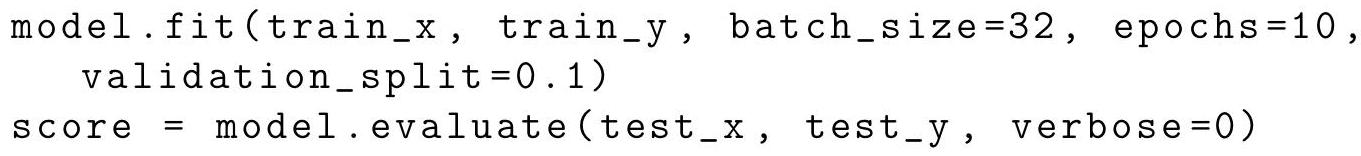
\includegraphics[max width=\textwidth]{2023_11_03_3a37fc63330e1b210712g-4}
\end{center}

\section*{(e) Experimentation}
i. Run the above training for 50 epochs. Using pyplot, graph the validation and training accuracy after every 10 epochs. Is there a steady improvement for both training and validation accuracy?

For accessing the required values while plotting, you can store the output of the fit method while training your network. Please refer to the code below.

\begin{center}
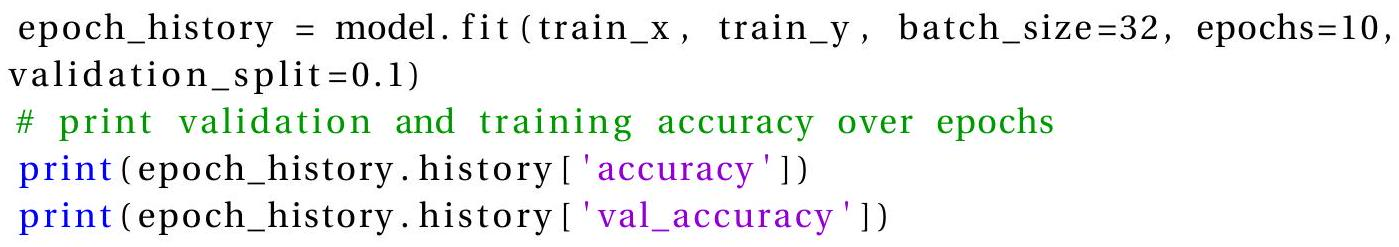
\includegraphics[max width=\textwidth]{2023_11_03_3a37fc63330e1b210712g-4(1)}
\end{center}

Make sure that your plot has a meaningful legend, title, and labels for X/Y axes.
ii. To avoid over-fitting in neural networks, we can 'drop out' a certain fraction of units randomly during the training phase. You can add the following layer (before the dense layer with 100 neurons) to your model defined in the function create\_cnn.

$$
\text { model. add (Dropout (0.5)) }
$$

Make sure you import Dropout from keras.layers! Now, train this CNN for 50 epochs.

Graph the validation and train accuracy after every 10 epochs.

This tutorial might be helpful if you want to see more examples of dropout with Keras.

iii. Add another convolution layer and maxpooling layer to the create\_cnn function defined above (immediately following the existing maxpooling layer). For the additional convolution layer, use 64 output filters. Train this for 10 epochs and report the test accuracy.

iv. We used a learning rate of 0.01 in the given create\_cnn function. Using learning rates of 0.001 and 0.1 respectively, train the model and report accuracy on test data-set. Use Dropout, 2 convolution layers and train for 10 epochs for this experiment.

\section*{(f) Analysis}
i. Explain how the trends in validation and train accuracy change after using the dropout layer in the experiments.

ii. How does the performance of CNN with two convolution layers differ as compared to CNN with a single convolution layer in your experiments?

iii. How did changing learning rates change your experimental results in part (iv)?

\begin{enumerate}
  \setcounter{enumi}{1}
  \item Random Forests for Image Approximation In this question, you will use random forest regression to approximate an image by learning a function, $f: \mathbb{R}^{2} \rightarrow \mathbb{R}$, that takes image $(x, y)$ coordinates as input and outputs pixel brightness. This way, the function learns to approximate areas of the image that it has not seen before.
\end{enumerate}

a. Start with an image of the Mona Lisa. If you don't like the Mona Lisa, pick another interesting image of your choice.

b. Preprocessing the input. To build your "training set," uniformly sample 5,000 random $(x, y)$ coordinate locations.

\begin{itemize}
  \item What other preprocessing steps are necessary for random forests inputs? Describe them, implement them, and justify your decisions. In particular, do you need to perform mean subtraction, standardization, or unit-normalization?
\end{itemize}

c. Preprocessing the output. Sample pixel values at each of the given coordinate locations. Each pixel contains red, green, and blue intensity values, so decide how you want to handle this. There are several options available to you:

\begin{itemize}
  \item Convert the image to grayscale

  \item Regress all three values at once, so your function maps $(x, y)$ coordinates to $(r, g, b)$ values: $f: \mathbb{R}^{2} \rightarrow \mathbb{R}^{3}$
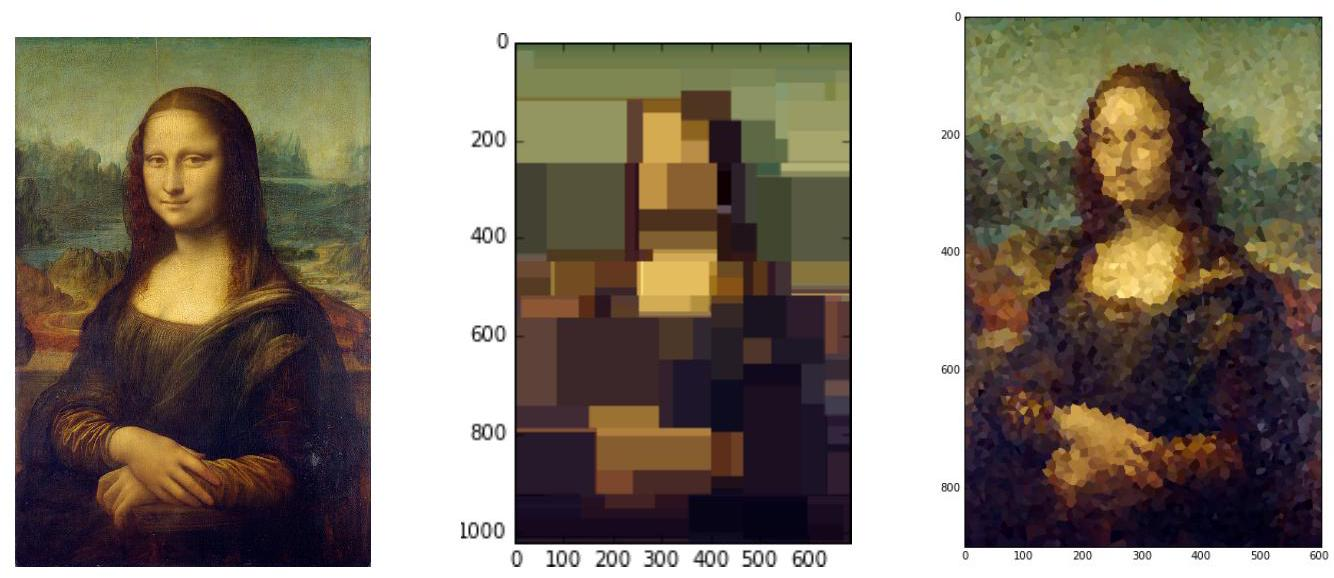
\includegraphics[max width=\textwidth, center]{2023_11_03_3a37fc63330e1b210712g-6}

\end{itemize}

Figure 1: Left: \href{http://tinyurl}{http://tinyurl} . com/mona-lisa-small Mona Lisa, Leonardo da Vinci, via Wikipedia. Licensed under Public Domain. Middle: Example output of a decision tree regressor. The input is a "feature vector" containing the $(x, y)$ coordinates of the pixel. The output at each point is an $(r, g, b)$ tuple. This tree has a depth of 7. Right: Example output of a $k$-NN regressor, where $k=1$. The output at each pixel is equal to its closest sample from the training set.

\begin{itemize}
  \item Learn a different function for each channel, $f_{\text {Red }}: \mathbb{R}^{2} \rightarrow \mathbb{R}$, and likewise for $f_{\text {Green }}, f_{\text {Blue }}$.
\end{itemize}

Note that you may need to rescale the pixel intensities to lie between 0.0 and 1.0. (The default for pixel values may be between 0 and 255, but your image library may have different defaults.)

What other preprocessing steps are necessary for random regression forest outputs? Describe them, implement them, and justify your decisions.

d. To build the final image, for each pixel of the output, feed the pixel coordinate through the random forest and color the resulting pixel with the output prediction. You can then use imshow to view the result. (If you are using grayscale, try imshow ( $Y, c m a p=$ 'gray') to avoid fake-coloring). You may use any implementation of random forests, but you should understand the implementation and you must cite your sources.

\section*{e. Experimentation.}
i. Repeat the experiment for a random forest containing a single decision tree, but with depths 1, 2, 3, 5, 10, and 15. How does depth impact the result? Describe in detail why.

ii. Repeat the experiment for a random forest of depth 7 , but with number of trees equal to $1,3,5,10$, and 100. How does the number of trees impact the result? Describe in detail why.

iii. As a simple baseline, repeat the experiment using a $k$-NN regressor, for $k=1$. This means that every pixel in the output will equal the nearest pixel from the "training set." Compare and contrast the outlook: why does this look the way it does? You may use an existing implementation of $k$-NN but make sure to cite your source.

iv. Experiment with different pruning strategies of your choice.

\section*{f. Analysis.}
i. What is the decision rule at each split point? Write down the 1-line formula for the split point at the root node for one of the trained decision trees inside the forest. Feel free to define any variables you need.

ii. Why does the resulting image look like the way it does? What shape are the patches of color, and how are they arranged?

\section*{WRITTEN EXERCISES}
\begin{enumerate}
  \item Maximum Margin Classifiers. Suppose we are given $n=7$ observations in $d=2$ dimensions. For each observation, there is an associated class label.
\end{enumerate}

a. Sketch the observations and the maximummargin separating hyperplane.

b. Describe the classification rule for the maximal margin classifier. It should be something along the lines of "Classify as Red if $\beta_{0}+\beta_{1} \mathbf{x}_{1}+$ $\beta_{2} \mathbf{x}_{2}<0$, and classify to Blue otherwise." Provide the values for $\beta_{0}, \beta_{1}$, and $\beta_{2}$.

\begin{center}
\begin{tabular}{lll}
$\mathbf{x}_{1}$ & $\mathbf{x}_{2}$ & $y$ \\
\hline
3 & 4 & Red \\
2 & 2 & Red \\
4 & 4 & Red \\
1 & 4 & Red \\
2 & 1 & Blue \\
4 & 3 & Blue \\
4 & 1 & Blue \\
\end{tabular}
\end{center}

c. On your sketch, indicate the margin for the maximal margin hyperplane.

d. Indicate the support vectors for the maximal margin classifier.

e. Argue that a slight movement of the seventh observation would not affect the maximal margin hyperplane.

f. Sketch a hyperplane that separates the data, but is not the maximum-margin separating hyperplane. Provide the equation for this hyperplane.

g. Draw an additional observation on the plot so that the two classes are no longer separable by a hyperplane.

\begin{enumerate}
  \setcounter{enumi}{1}
  \item Ensemble Models. In this question, we will get more hands-on experience using ensemble models. Throughout, suppose our inputs live in two-dimensional space. Formally, for all $\mathbf{x} \in \mathbb{R}^{2}$, let $\mathbf{x}_{1}$ and $\mathbf{x}_{2}$ be the first and second components of the input vector, respectively. Suppose we have a binary classification dataset consisting of four labeled datapoints, with labels $y^{(i)} \in\{0,1\}$ :
\end{enumerate}

\begin{itemize}
  \item $\mathbf{x}^{(1)}=[0,2]^{\top}, y^{(1)}=1$

  \item $\mathbf{x}^{(2)}=[2,0]^{\top}, y^{(2)}=1$

  \item $\mathbf{x}^{(3)}=[0,0]^{\top}, y^{(3)}=0$

  \item $\mathbf{x}^{(4)}=[-2,2]^{\top}, y^{(4)}=0$

\end{itemize}

\begin{center}
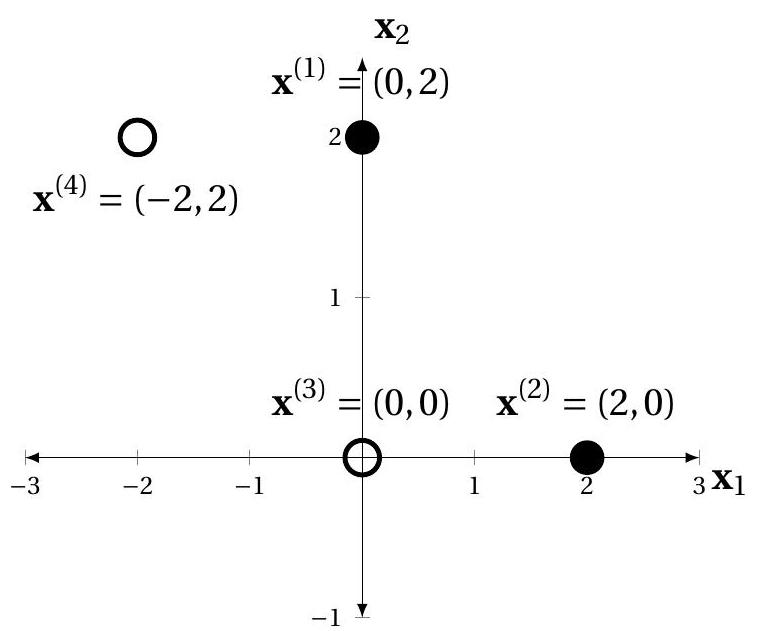
\includegraphics[max width=\textwidth]{2023_11_03_3a37fc63330e1b210712g-8}
\end{center}

As you can see in the plot above, this dataset is diagonally linearly separable, meaning there is a diagonal linear decision boundary that will perfectly classify the points with label 1 (filled in black) and those with label 0 (not filled).

a. Let $g: \mathbb{R}^{2} \mapsto\{0,1\}$ be a binary classifier of the form $g(x)=\mathbf{1}\left\{\mathbf{x}_{j}>c\right\}$, where $\mathbf{1}$ is an indicator function (equal to one if its input is true and zero otherwise), $j \in\{1,2\}$ is a coordinate, and $c \in \mathbb{R}$ is a threshold value. In other words, the function $g$ looks at some coordinate $j$ of $\mathbf{x}$ and
returns one if it is greater than $c$, and zero otherwise. Note that we can view $g$ as a decision tree of depth one. We will refer to a $g$ of this form as a threshold function.

There exists an ensemble model $f(\mathbf{x})=\sum_{t=1}^{T} \alpha_{t} g_{t}\left(\mathbf{x}^{(i)}\right)$ consisting of a weighted average of $T$ threshold functions $g_{t}$ with weights given by $\alpha_{t} \in \mathbb{R}$ such that the training error of $f$ is zero (i.e., for all points $\mathbf{x}^{(i)}$ in the training set, $y^{(i)}=\mathbf{1}\left\{f\left(\mathbf{x}^{(i)}\right)>0.5\right\}$ ). In other words, we can ensemble shallow decision trees that represent only horizontal or vertical decision boundaries into a more expressive classifier with a diagonal decision boundary. Find the functions $g_{t}$ and the weights $\alpha_{t}$ that yield an ensemble $f$ with a classification error of zero on the training set.

(Hint: there exists a solution with $T=3$. Also, the weights can all be equal.)

b. On the original plot above or on a duplicate, draw the decision boundary of this ensemble and clearly indicate on which side your ensemble would predict a label of +1 or 0 .


\end{document}